In questo esperimento, \'{e} stato attaccato al sensore un filo con appeso un oggetto di 0.25Kg. 
Il braccio \'{e} stato posizionato in modo tale che la forza peso gravasse solo su un asse del sensore alla volta. 
In Figura \ref{boh}, viene mostrato il setup per l'esperimento.
Dopo aver azzerato il sensore, per verificarne la reattivit\'{a}, il filo \'{e} stato tagliato di netto. 
Il taglio del filo \'{e} un ottimo modo per `simulare' un cambiamento di forza istantaneo.
\begin{figure}[H]
    \centering
    \includegraphics*[width=0.80\textwidth]{images/z_cut.png}
    \caption{Andamento taglio del filo lungo l'asse z}
    \label{fig:z_cut}
\end{figure}
In Figura \ref{fig:z_cut} viene mostrato l'andamento della forza rilevata dal sensore lungo l'asse z. 
Si pu\'{o} notare che, fino a quando il filo \'{e} attaccato al sensore, la forza rilevata \'{e} circa zero. 
Questo perch\'{e} il sensore \'{e} stato azzerato quando l'oggetto era gi\'{a} stato appeso. 
Dopo circa 15 secondi, il filo viene tagliato. In questo istante il sensore rileva per una frazione di secondo una forza di circa 1.5N 
(probabilmente dovuta ad un taglio non sufficientemente netto), per poi assestarsi al valore reale della forza rilevata, 
ossia circa -2.5N. 
Tale esperimento \'{e} stato ripetuto anche per gli altri due assi con esiti leggermente migliori. 
I risultati vengono mostrati in Figura \ref{fig:cut_results}.
\begin{figure}[H]
    \centering
    \begin{subfigure}[b]{0.80\textwidth}
        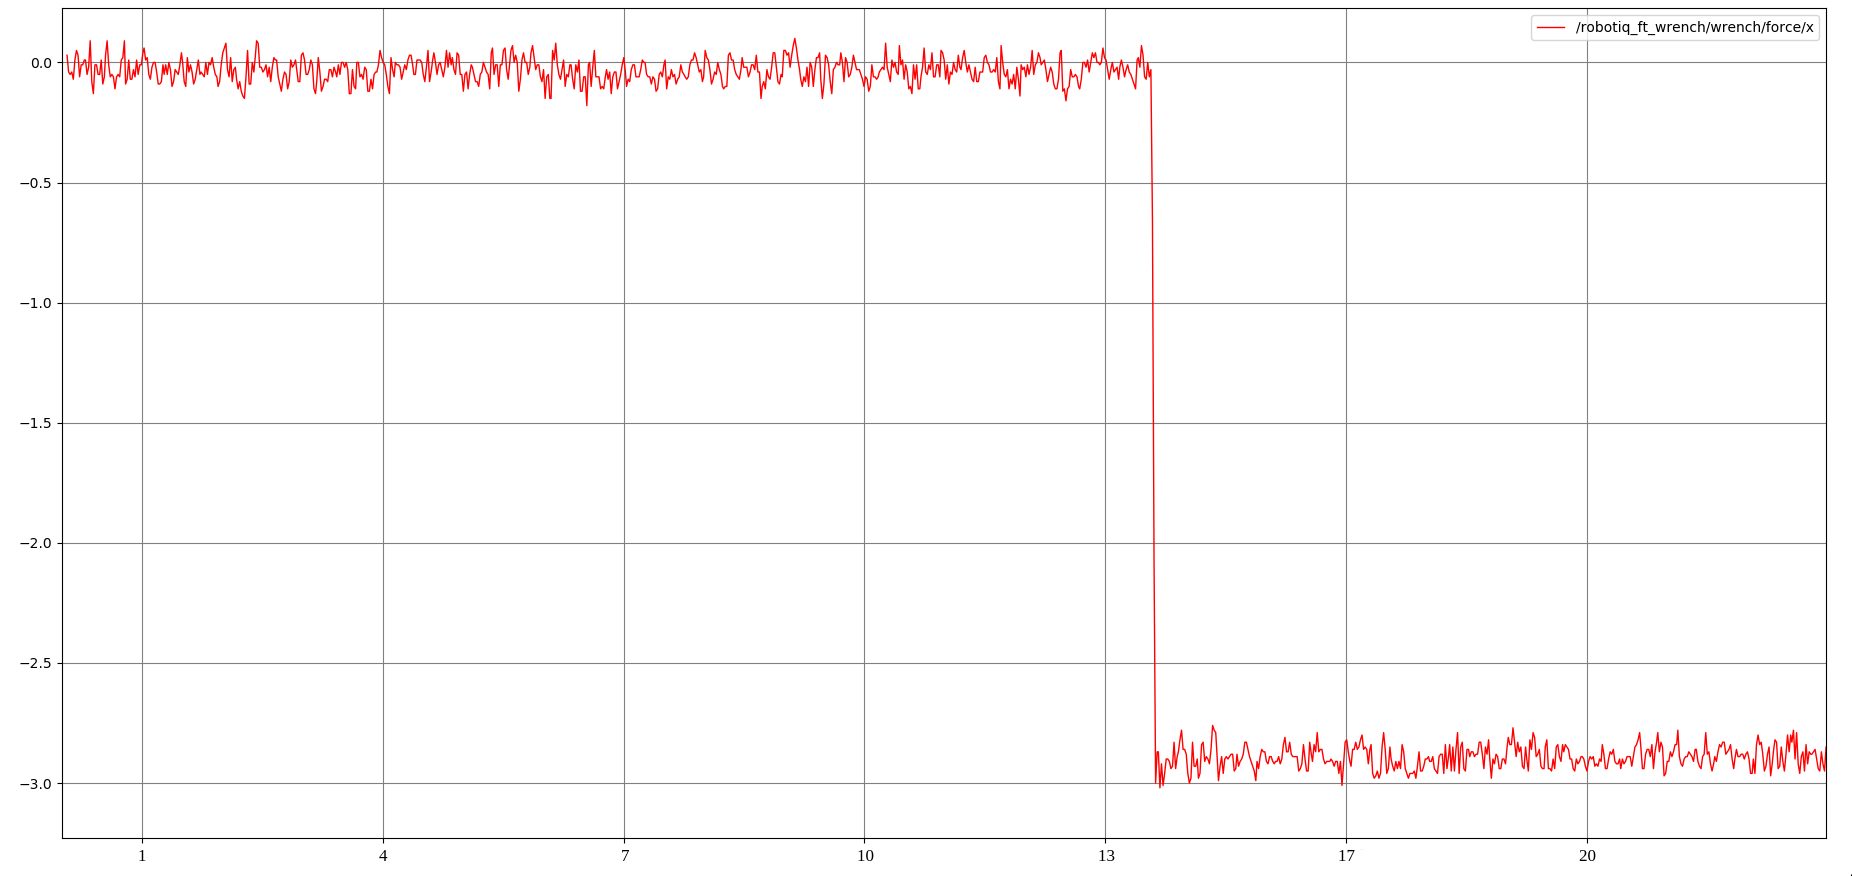
\includegraphics[width=\textwidth]{images/x_cut.png}
        %\caption{}
        \label{fig:x_cut}
    \end{subfigure}
    ~ %add desired spacing between images, e. g. ~, \quad, \qquad, \hfill etc. 
      %(or a blank line to force the subfigure onto a new line)
    \begin{subfigure}[b]{0.80\textwidth}
        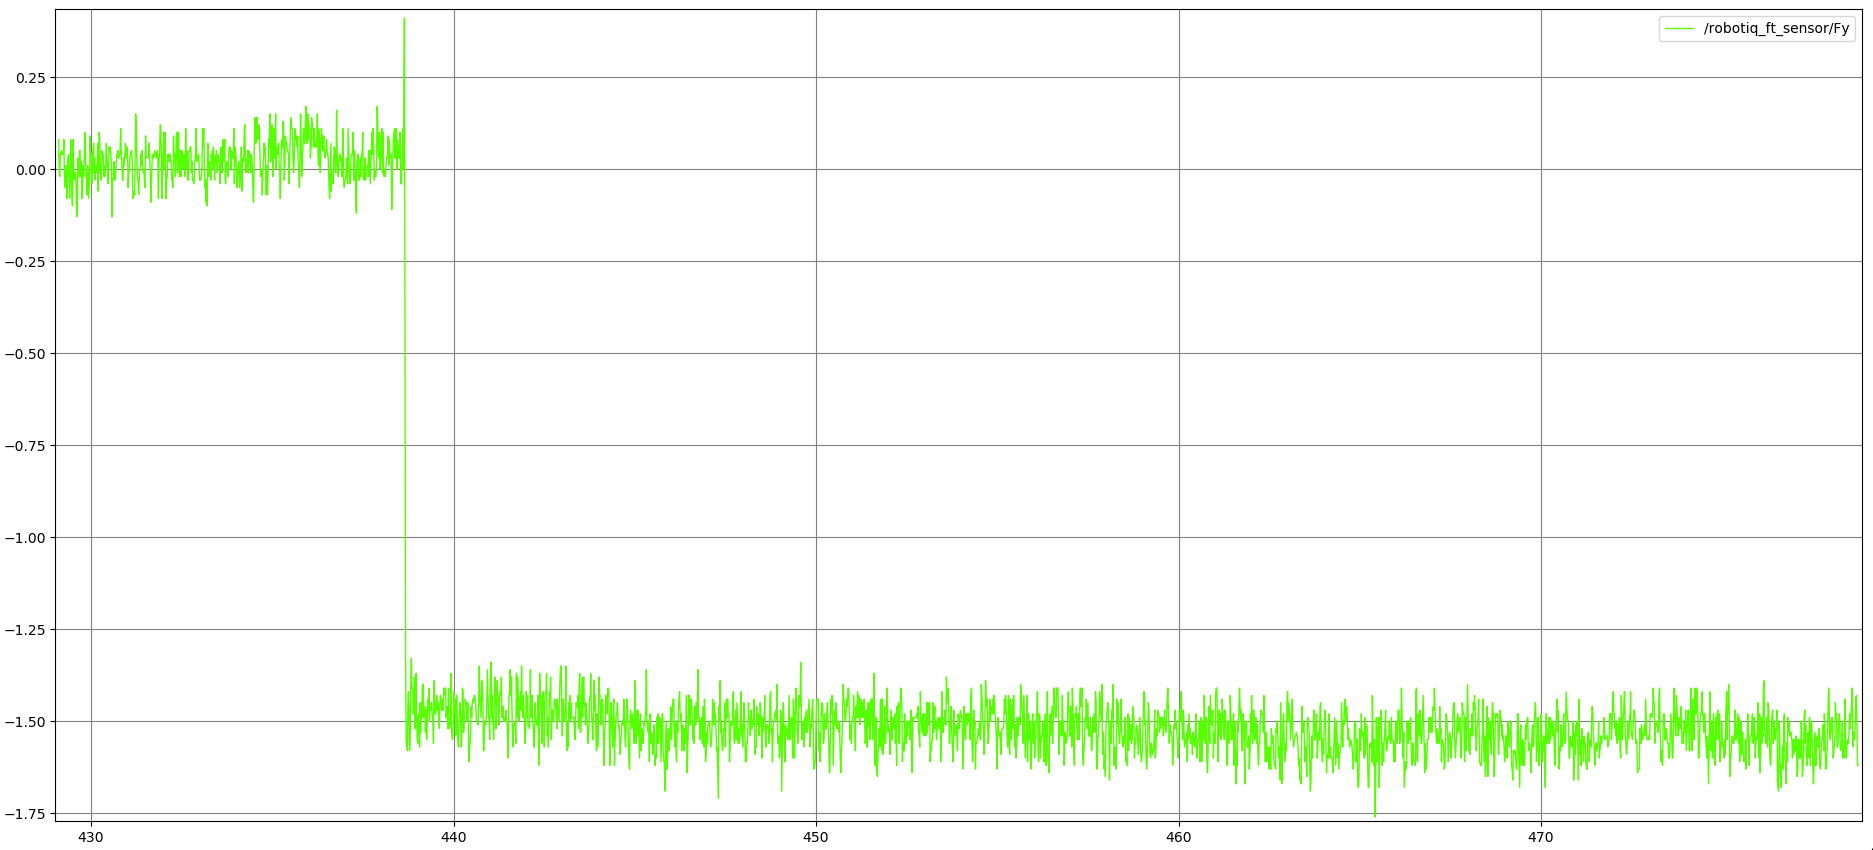
\includegraphics[width=\textwidth]{images/y_cut.png}
        %\caption{}
        \label{fig:y_cut}
    \end{subfigure}
    \caption{Andamento esperimento lungo x e y}\label{fig:cut_results}
\end{figure}
